% Created 2022-02-18 sex 14:36
% Intended LaTeX compiler: pdflatex
\documentclass[letterpaper, 11pt]{article}
                      \usepackage{lmodern} % Ensures we have the right font
\usepackage[T1]{fontenc}
\usepackage[utf8]{inputenc}
\usepackage{graphicx}
\usepackage{amsmath, amsthm, amssymb}
\usepackage[table, xcdraw]{xcolor}
\definecolor{bblue}{HTML}{0645AD}
\usepackage[colorlinks]{hyperref}
\hypersetup{colorlinks, linkcolor=blue, urlcolor=bblue}
\usepackage{titling}
\setlength{\droptitle}{-6em}
\setlength{\parindent}{0pt}
\setlength{\parskip}{1em}
\usepackage[stretch=10]{microtype}
\usepackage{hyphenat}
\usepackage{ragged2e}
\usepackage{subfig} % Subfigures (not needed in Org I think)
\usepackage{hyperref} % Links
\usepackage{listings} % Code highlighting
\usepackage[top=1in, bottom=1.25in, left=1.55in, right=1.55in]{geometry}
\renewcommand{\baselinestretch}{1.15}
\usepackage[explicit]{titlesec}
\pretitle{\begin{center}\fontsize{20pt}{20pt}\selectfont}
\posttitle{\par\end{center}}
\preauthor{\begin{center}\vspace{-6bp}\fontsize{14pt}{14pt}\selectfont}
\postauthor{\par\end{center}\vspace{-25bp}}
\predate{\begin{center}\fontsize{12pt}{12pt}\selectfont}
\postdate{\par\end{center}\vspace{0em}}
\titlespacing\section{0pt}{5pt}{5pt} % left margin, space before section header, space after section header
\titlespacing\subsection{0pt}{5pt}{-2pt} % left margin, space before subsection header, space after subsection header
\titlespacing\subsubsection{0pt}{5pt}{-2pt} % left margin, space before subsection header, space after subsection header
\usepackage{enumitem}
\setlist{itemsep=-2pt} % or \setlist{noitemsep} to leave space around whole list
\author{Vinicius Faria}
\date{\today}
\title{Cálculo 2\\\medskip
\large \emph{Anotações Práticas}}
\hypersetup{
 pdfauthor={Vinicius Faria},
 pdftitle={Cálculo 2},
 pdfkeywords={},
 pdfsubject={},
 pdfcreator={Emacs 27.2 (Org mode 9.5.2)}, 
 pdflang={English}}
\begin{document}

\maketitle
\tableofcontents

Esse pdf não possui propósito comercial, feito somente para fins educativos, foi baseado e contêm partes do livro: Calculo III - CEDERJ. Contato: artixsproductions@gmail.com

\section{Funções Vetoriais}
\label{sec:org1ea2024}
Funções cuja imagem gerada é um vetor. \(\realbb{R}^2 \ e \ \realbb{R}^3\) são chamadas \textbf{funções coordenadas} e t é denominado \textbf{variável livre}

\begin{center}   $\alpha(t) = (2t+1, 1-t)$ \end{center}

\subsection{Esboço de curvas}
\label{sec:org5849d6e}
Para esboçar curvas, isolar o x e y (e potencialmente z) em função de t, formando a imagem da curva. A curva abaixo descreve um círculo.

\begin{center} $\begin{cases} x(t) = \sin (t) \\ y(t) = \cos(t) \end{cases}$ \end{center}

\subsection{Equações paramétricas de retas}
\label{sec:orge694608}
Dado uma curva que passa por A e B, é possível definir sua função utilizando:

\begin{center} $\alpha (t) = (1-t)A + tB = A + t(B-A)$ \end{center}

Interpretação geométrica: parametrização da reta que contém o ponto A e é parelela ao vetor não nulo (B-A)

\subsection{Parametrizações}
\label{sec:orgf522ea3}
Uma função vetorial é uma \uline{parametrização} da curva que é a imagem da função. Uma curva pode ser parametrizada de várias maneiras, como círculos.

\subsection{Limites e Continuidade}
\label{sec:org5e5866a}
Resumidamente, para calcular limites de funções vetoriais, basta calcular o limite de cada função de coordenada separadamente.

Da mesma forma, para verificar a continuidade da função vetorial, basta conferir que todas as funções de coordenadas sejam contínuas.

\textbf{OBS:} Uma função é contínua quando em seu domínio:
\begin{itemize}
\item Não possui assíntotas verticais
\item Não possui "furos"
\item Não possui "pulos"
\end{itemize}
\textbf{OBS2:} \(\Vert \alpha (t) \Vert\) denota o módulo do vetor.
\subsection{Derivadas de funções vetoriais}
\label{sec:org779d0a1}
A derivada de uma função vetorial é interpretada como o \textbf{vetor tangente ao traço de \(\alpha\) no ponto \(\alpha(a)\)}. Obtida por derivar cada coordenada separadamente. \textbf{Podemos calcular},
\textbf{por exemplo, o ângulo entre 2 curvas em um dado ponto através do ângulo das 2 derivadas no dado ponto.}

\begin{center} $\alpha(t)' = (\alpha_1'(t), \alpha_2'(t),...)$ \end{center}

Quando a derivada é \(\theta\), gráfico apresenta uma "cúspide". Essa cúspide, no contexto de funções vetoriais, \textbf{não significa que a função é indiferenciável!!!} E sim que o vetor da derivada é equivalente ao vetor nulo.
\begin{center}
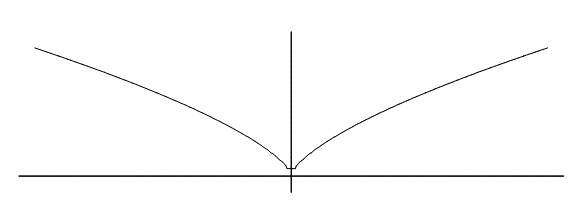
\includegraphics[width=.9\linewidth]{./img/cuspide.png}
\end{center}

\subsubsection{Retas tangentes}
\label{sec:org3b5cd79}
Para calcular a reta tangente à função vetorial no ponto a, a derivada é a reta e as coordenadas de \(\alpha\) no ponto a é o ponto inicial.

\begin{center} $r(t) = t\alpha'(a) + \alpha(a)$ \end{center}

No caso de \textbf{coordenadas polares} (tomada por comprimento e angulo de um vetor em vez de coordenadas usuais), tomar como base, e depois procedir normalmente:

\begin{center} $\alpha(\theta) = (r(\theta)\cos\theta, r(\theta)\sin\theta)$ \end{center}

\textbf{Exemplo:}

\(\alpha(t) = (t^2, 3t+1) \rightarrow \alpha'(t) = (2t, 3)\)

Então, a reta no ponto \(t = -1\) será

\(t(2\cdot-1, 3) + ((-1)^2,3(-1)+1) \rightarrow (2t+1, 3t+4)\)

No geogebra:
\begin{center}
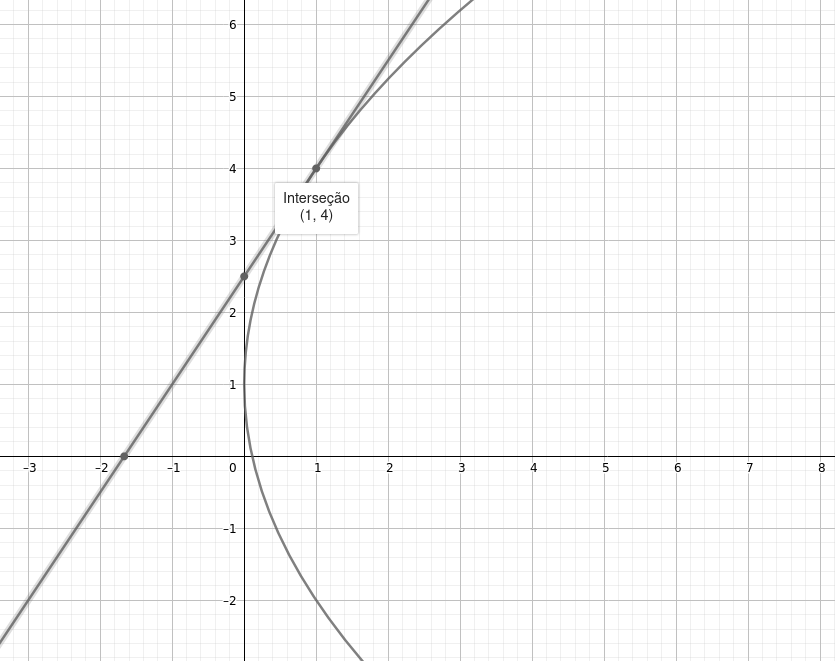
\includegraphics[width=.9\linewidth]{./img/tangente.png}
\end{center}

\textbf{Outro exemplo importante}

Dado a curva \(\alpha(t) = (t^3 +3t, t^2+4t)\), encontrar ponto(s) onde a curva é tangente à reta \(r(t) = (3t+3,t-4)\)

Passo-a-passo: Derivar a curva, encontrar pontos em que essa derivada é paralela ao vetor diretor da reta, isto é: \(\alpha'(t) = \lambda(3,1)\). Solucionar num sistema linear. (Gabarito \(t = -1, t = 3\))

\subsection{Integrais de funções vetoriais}
\label{sec:orga5b5c63}
Integrar uma função vetorial é feito da mesma maneira que na derivação: integrando um a um. Realizando a integração indefinida, obtemos a função primitiva de cada uma das coordenadas, sendo útil para descobrir a velocidade através da aceleração, por exemplo.
Por outro lado, a integração definida resulta num vetor. Uma nomenclatura comum no caso da integração até \(\realbb{R}^3\) é separar as coordenadas em \(\vec{i}, \vec{j} \ e \ \vec{k}\) para representar x,y e z.

\begin{center} $\int_{a}^{b} \alpha(t) \ dt = \int_{a}^{b} \alpha_1(t) \ dt \ \vec{\textbf{i}} + \int_{a}^{b} \alpha_2(t) \ dt \ \vec{\textbf{j}} +  \int_{a}^{b} \alpha_3(t) \ dt \ \vec{\textbf{k}}  $ \end{center}

\subsubsection{Comprimento de uma curva}
\label{sec:orge377f53}
Tomando a ideia de módulo de vetores com o somatório da integral, levando em conto que \(\alpha\) é uma função de classe \(C^1\) (Continua e derivável em todos os pontos) tomamos a fórmula:

\begin{center} $L(\alpha) = \int_{a}^{b} |\alpha'(t)| dt \ , \ |\alpha'(t)| = \sqrt{(\alpha_1'(t))^2 + (\alpha_2'(t))^2}$ \end{center}

\subsubsection{Curvas em coordenadas polares}
\label{sec:orgadb780d}
A fórmula do comprimento de uma curva dada, caso \(r(\theta)\) seja de classe \(C^1\), pela equação \(r = r(\theta)\) é:

\begin{center} $L =\int_{a}^{b} \sqrt{(\dfrac{dr}{d\theta})^2 + r^2 d\theta}$ \end{center}

A fórmula da área da região delimitada por \(0 \le r \le r(\theta), a < \theta < b\) é

\begin{center} $A =\frac{1}{2} \int_{a}^{b} r(\theta)^2 d\theta$ \end{center}

\begin{center}
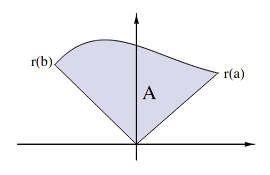
\includegraphics[width=.9\linewidth]{./img/areapolar.png}
\end{center}

\section{Funções reais de várias variáveis}
\label{sec:org71880e9}
\subsection{Duas variáveis}
\label{sec:org8a44844}
Funções de 2 variáveis são do tipo \(f: A \subset \realbb{R}^2 \rightarrow \realbb{R}\), cuja lei de definição tem a forma \(z = f(x,y)\), com x e y variáveis independentes. A função gera um espaço tridimensional, muitas vezes formando curvas ou formas específicas.

\begin{center}
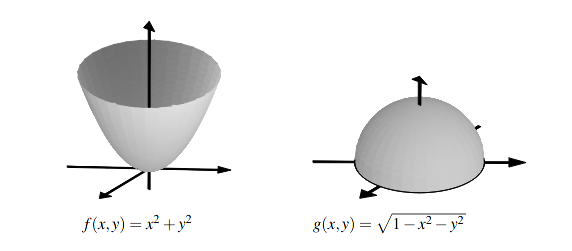
\includegraphics[width=.9\linewidth]{./img/2varex.png}
\end{center}

O seu domínio é bidimensional (pois não há z), determinado pelas regras usuais. Ex. Raiz quadrada >= 0, logaritmo > 0, etc.

\subsection{Três ou mais variáveis}
\label{sec:org624287e}
Seu gráfico é \(\realbb{R}^n\), com \(n \ge 4\), portanto não são esboçáveis na mão. Porém, é possível esboçar domínios de funções de três variáveis, que resultam em um espaço tridimensional.

Ex. \(w = f(x,y,z) = \sqrt{4-x^2-y^2-z^2}\) tem o domínio \(A =\) \{ \((x,y,z) \in \realbb{R}^3; x^2 + y^2 + z^2 \le 4}\) \}. Que é equivalente aos pontos interiores de uma esfera de raio 2.

\subsection{Gráficos de funçoes simples de 2 variáveis}
\label{sec:org5a44082}
\subsubsection{Superfícies quadráticas}
\label{sec:org243222f}
Parabolóides, elipsóides.. Ex: \(f(x,y) = \sqrt{36-9x^2-4y^2}\), que resulta em \(\frac{x^2}{4} + \frac{y^2}{9} + \frac{z^2}{36} = 1\), resultando em uma elipsóide com \(z \ge 0\):

\begin{center}
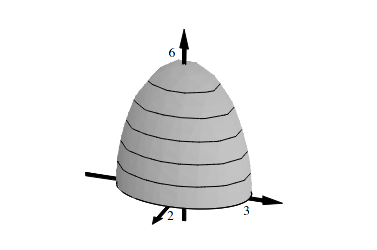
\includegraphics[width=.9\linewidth]{./img/elipsoide.png}
\end{center}

\subsubsection{Superfícies cilíndricas}
\label{sec:org8f5ee42}
Funções em que há apenas x ou y. Plotar o gráfico normalmente e depois apenas extender ele ao longo do eixo (todos os planos da variável que falta)

\begin{center}
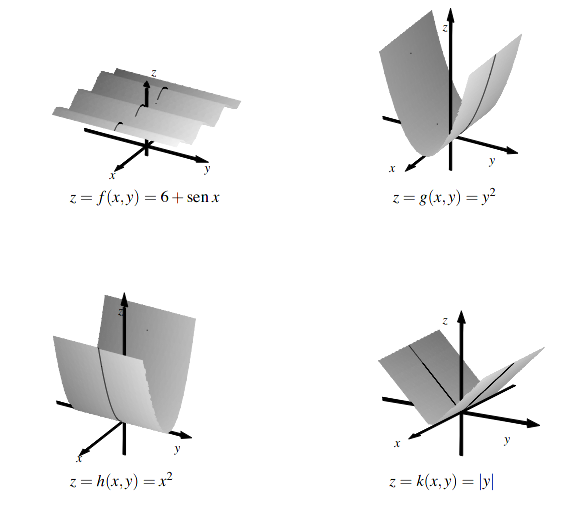
\includegraphics[width=.9\linewidth]{./img/cilindricas.png}
\end{center}

\subsubsection{Superfícies de revolução}
\label{sec:orgeaeca34}
Funções com forma de \(z= f(x,y) = g(x^2+y^2)\). Para esboçar o gráfico, esboçar gráfico da função em \(z=f(x,0)\) e girar a curva ao redor do eixo 0z

\begin{center}
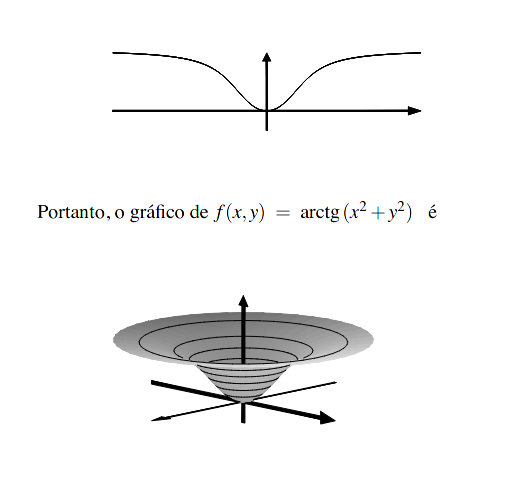
\includegraphics[width=.9\linewidth]{./img/revolucao.png}
\end{center}

\subsection{Esboçando gráficos}
\label{sec:org03b99ed}
\subsubsection{Funções g(x) ou h(y)}
\label{sec:org05c1eb2}
As leis da forma \(f(x,y) = g(x)\) ou \(f(x,y) = h(y)\), são chamadas \emph{invariantes}, uma vez que fixado um x ou y, alternar a outra coordenada nao altera a imagem. Assim:

\begin{center} $(a,b+t, f(a,b) = (a,b+t,f(a,b+t))$ \end{center}

Em termos gerais, é so montar um gráfico em \(\mathbb{R}^2\) e "deslizar" a imagem para formar a superfície.

\begin{center}
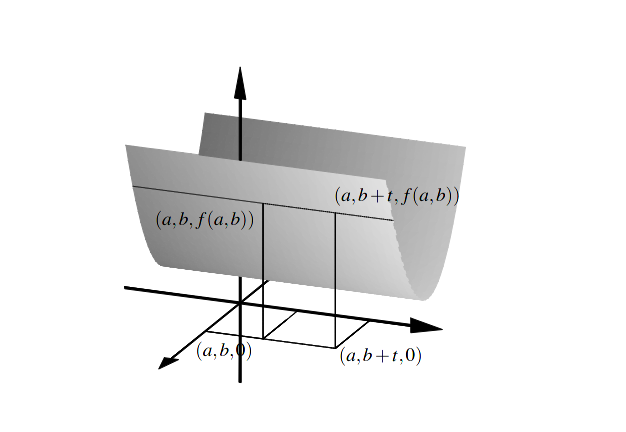
\includegraphics[width=.9\linewidth]{./img/esbocar1.png}
\end{center}

\subsubsection{Caso g(x) + h(y)}
\label{sec:org042b7be}
No caso de funções \(f(x,y) = g(x) + h(y)\), de forma que x e y são separaveis em duas parcelas, como \(f(x,y) = x^2+\frac{y}{2} + 1\). Em termos gerais, observamos os casos \(f(x,y) = (x,c)\) e
\(f(x,y) = (d,y)\), dado c e d constantes, e analisamos o gráfico em \(\mathbb{R}^2\) para x e y separadamente. Assim, plotando os dois, "deslizamos" um gráfico sobre outro, criando o gráfico.

\begin{center}
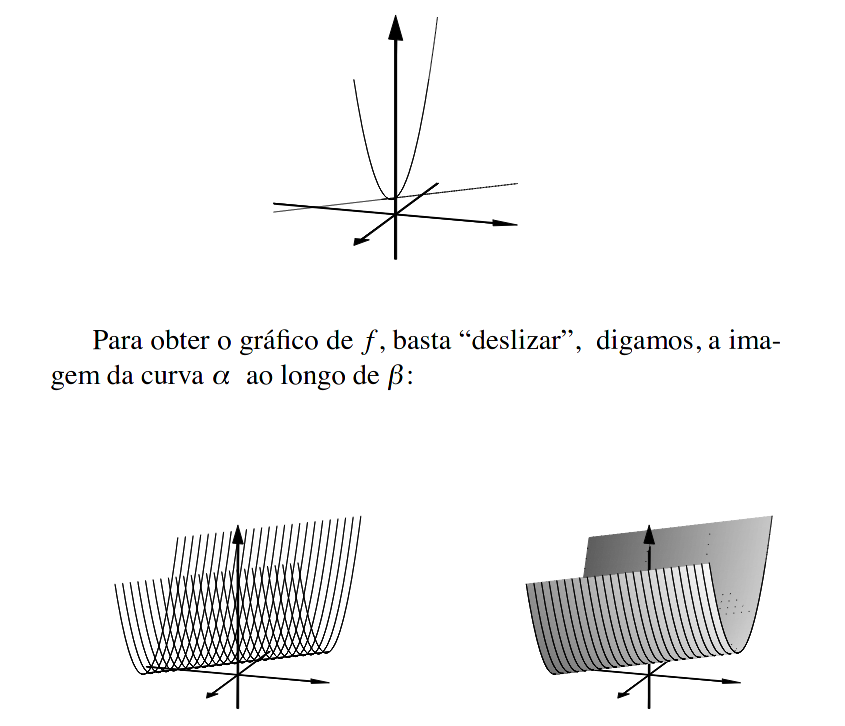
\includegraphics[width=.9\linewidth]{./img/esbocar2.png}
\end{center}

\subsection{Conjuntos de nível}
\label{sec:orgb47df39}
Basicamente conjuntos que agrupam imagens iguais para uma mesma função.
\subsubsection{Conjunto de nível}
\label{sec:org945d94e}
Quando temos uma função plana (de 1 variável) há apenas pontos representando elementos com a mesma imagem. Dado \(f(x) = x^2+2x\) e o conjunto de nível (\(f^{-1}(a)\)), temos:

\begin{center} $f^{-1}(3) = \{-1,3\}$ \end{center}

Onde -1 e 3 possuem a mesma imagem, no caso 3.

\subsubsection{Curvas de nível}
\label{sec:org6e83089}
Quando lidamos com conjuntos de nível em funções de 2 variável, obtemos \emph{curvas de nível}, cuja imagem podem ser elementos em \(\mathbb{R}^2\), como retas, circulos, pontos, etc. Assim,

\begin{center} $f(x,y) = b$ \end{center}

Assim, projetamos z=b,  e resolvemos o sistema no estilo de \(z = f(x,y)\), obtendo um dos elementos descritos. Nesse caso, denominamos uma "Curva de nível b"

Por exemplo, temos \(f(x,y) = z = b = x^2 +y^2 -4y+2\). No caso de z=2, por exemplo, temos \(4 = (x-2)^2 + y^2\), que resulta numa circuferência com centro em (2,0) e raio 2.

\begin{center}
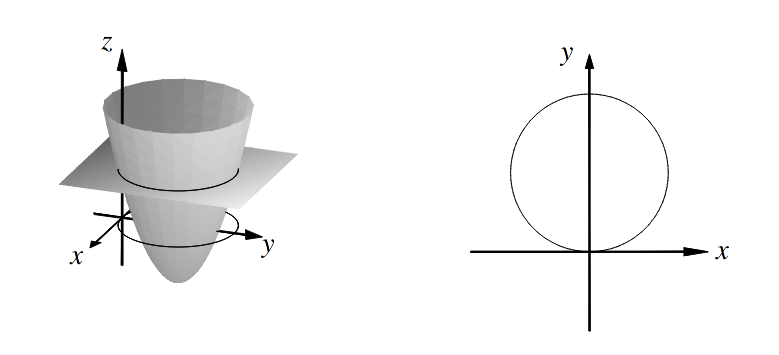
\includegraphics[width=.9\linewidth]{./img/curvanivel.png}
\end{center}

Para um mesmo b, podem haver várias curvas de nível, como na equação \(\frac{4x^2y}{x^4+y^2} = 1\).

\begin{center}
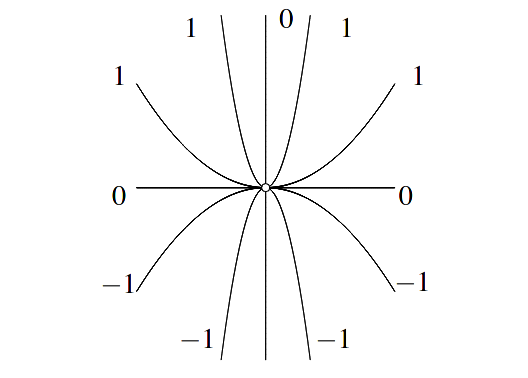
\includegraphics[width=.9\linewidth]{./img/nivelmultipla.png}
\end{center}

\subsubsection{Superfícies de nível}
\label{sec:org10b8a3d}
Para funções de 3 variáveis, dado \(w = f(x,y,z) = x^2+y^2-z^2\), ou seja fixando um w, obtemos uma \textbf{superfície}, assim como observada na geometria analítica.

No caso da equação dada, se \(c<0\), resulta numa hiperbolóide de 2 folhas, \(c=0\) num cone, e \(c>0\) uma hiperbolóide de uma folha.

\begin{center}
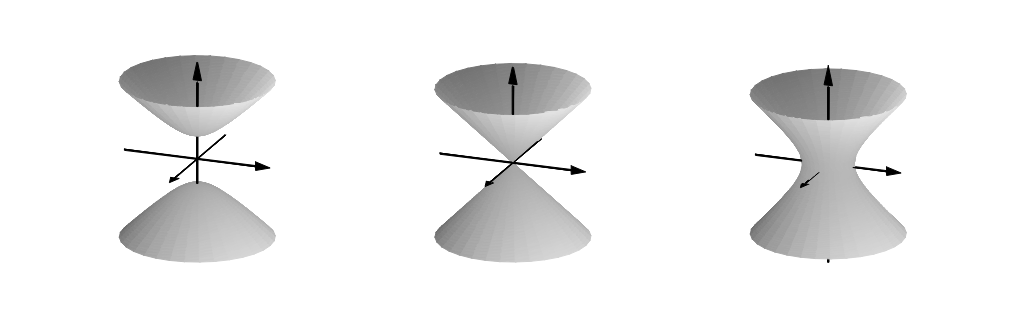
\includegraphics[width=.9\linewidth]{./img/supnivel.png}
\end{center}

\subsection{Limites}
\label{sec:org43928a9}
Exploramos agora limites de funções de 2 ou mais variáveis.

\subsubsection{Pontos de acmulação}
\label{sec:org2183089}
Determinar quais pontos são elegíveis para tomar o limite da função. Dado um ponto P em um conjunto D. Caso P estiver no mesmo ambiente \(\mathbb{R}^n\) que D, ele pode ser um ponto de acumulação de D,
mesmo que não necessariamente pertença ao seu conjunto. Imaginamos um "halo" em volta de P, se ele encosta em D, pode ser um ponto de acumulação. Não irei entrar em definições aqui, mas
tem-se como exemplo:

\begin{center} $P = (0,1,0), D = \{(x,y,z) \in \mathbb{R}^3; x^2 + y^2 > 1\}$, P é um ponto de acumulação. $\\ P=(0,0,0), D = \{(x,y,z) \in \mathbb{R}^3; x^2 + y^2 > 1\}$, P não é PA. \end{center}

\subsubsection{Limite de funções 2 ou mais variáveis}
\label{sec:org8723cfc}
Definição é a mesma, estruturalmente, do que a observada em limties de funções de uma variável.

\subsubsection{Propriedade dos limites}
\label{sec:orgab765fa}
As propriedades de limites também continuam as mesmas. Dado \(\lim_{(x,y) \to (a,b)} f(x,y) = L\) e \(\lim_{(x,y) \to (a,b)} g(x,y) = M\):

\begin{center}
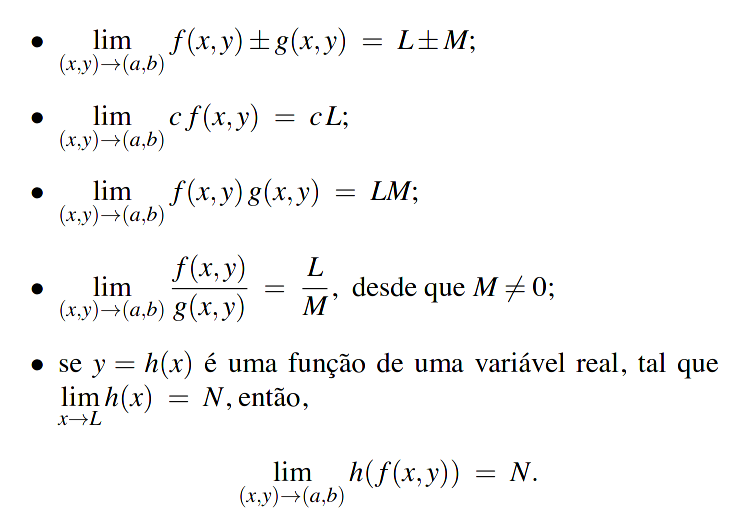
\includegraphics[width=.9\linewidth]{./img/proplim.png}
\end{center}

\subsubsection{Encontrando limites}
\label{sec:org33323ef}
\begin{enumerate}
\item Coordenadas polares
\label{sec:orge8545e2}
Em alguns casos, podemos converter x e y para coordenadas polares para chegar na resolução correta. Assim, \(x = r \cos\theta, y= r\cos\theta, x^2 + y^2 = r^2\). Quando convertemos, aplicar o limite
correto para r segundo a expressão anterior. Pode-se fazer L'Hopital e outras técnicas de integração de 1 variável. Por exemplo:

\begin{center} $\lim_{(x,y) \to (0,0)} \frac{\sin xy}{\sqrt{x^2+y^2}} = lim_{r \to 0} \frac{\sin(r^2 \cos\theta \sin\theta}{r}$ \end{center}

Assim, aplica-se L'hopital em r, e o resultado sera 0.
\item Manipulação algébrica
\label{sec:orgaff3030}
A primeira maneira de encontrar limites dessas funções seria a manipulação algébrica, de maneira que possibilite a substituição direta na função dada. Trabalhar com o denominador e
propriedades para encontrar o resultado.

\item Substituição
\label{sec:org8b7cf55}
\begin{center}
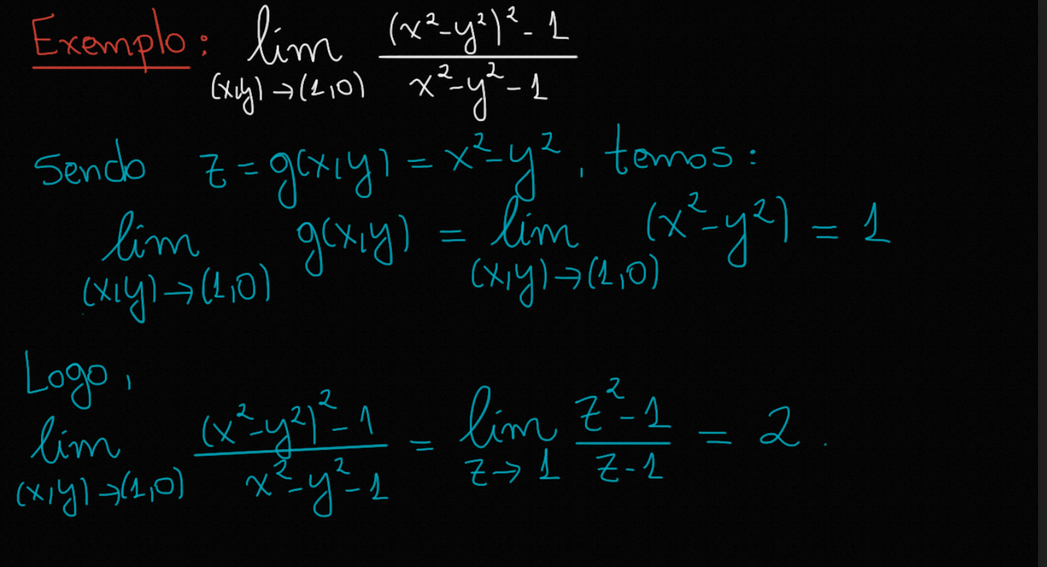
\includegraphics[width=.9\linewidth]{./img/limsubst.png}
\end{center}
\item Teorema do confronto
\label{sec:org4aebcf7}
Em termos práticos, dado que g é função limitada, ou seja, \(f(x,y) \le g(x,y) \le h(x,y)\) e os limites de f e h em \((a,b)\) sejam \(L\), então: \(\lim_{(x,y) \to (a,b)} g(x,y) = L\).

\begin{center} $\lim_{(x,y) \to (0,0)} \frac{\sin(x+y)}{x+y} = 1$ \end{center}

Outra adaptação desse teorema:
Dado \(\lim_{(x,y) \to (a,b)} f(x,y) = 0\), e \(\exists M > 0, |g(x,y)| < M\), então, \(\lim_{(x,y) \to (a,b)} f(x,y)g(x,y) = 0\).

Como exemplo:

\begin{center} \(\lim_{(x,y) \to (0,0)} \frac{x^2y}{x^2+y^2} = 0\), pois: \(\\ 0 \le x^2 \le x^2+y^2\) \(\\ 0 \le \frac{x^2}{x^2 + y^2} \le 1\). Assim, \(\\\) \(|g(x,y)| =  \frac{x^2}{x^2+y^2} \le 1\). Como lim y = 0, temos que o limite é 0.
\end{enumerate}

\subsubsection{Existência do limite}
\label{sec:orga70c7c8}
Para confirmar a existência de limites dados, inserimos funções vetoriais. Assim, dado \(\lim_{t \to t_o} \alpha_1(t) = (a,b) = \lim_{t \to t_0} \alpha_2(t)\), \(\lim_{t \to t_o} f(\alpha_1(t) = \lim_{t \to t_o} f(\alpha_2(t) = L\),
para o limite existir.

Em termos praticos, dado \(\lim_{(x,y) \to (a,b)} f(x,y)\), o limite deve ser o mesmo substituindo para diferentes funções vetoriais \(\alpha(t)\) que resultam no mesmo vetor. Como \(\alpha(t) = (t,b); \alpha_2(t) = (a,t), \alpha_3(t) = (\beta t, \gamma t)\), a primeira com t tendendo a a, e a segunda, a b, etc.

Tomando o exemplo \(f(x,y) = \frac{xy}{x^2+y^2}\):

\begin{center}
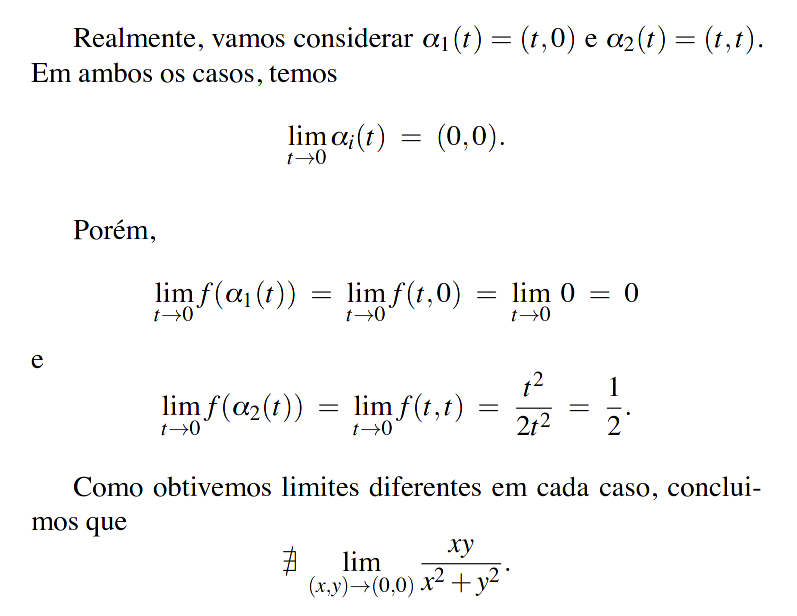
\includegraphics[width=.9\linewidth]{./img/exlim.png}
\end{center}

\textbf{OBS:} No caso de \(f=(t,t)\) devemos manipular a funções das duas coordenadas para tornar t substituível sem indeterminações. Ex - \(f(x) = \frac{xy^2}{x^4+y^4}\), fazemos \(\alpha(t) = (t^2,t)\).

Esse método de conferir deve-se ao fato de que, em funções de 2 ou mais variáveis, o limite deve ser o mesmo para os diversos "feixes" que aproximam em \((a.b)\), análogo aos limites laterais
estudados em calculo I.

\subsection{Continuidade}
\label{sec:orge0fd8e3}
Não há novidades no caso de Cálculo II. Dada a função \(f: A \subset \mathbb{R}^2 \to \mathbb{R}\), ela será contínua no ponto \((a,b)\) de acumulação de A caso:
\begin{itemize}
\item \((a,b) \in A\)
\item \(lim_{(x,y) \to (a,b)} = f(a,b)\)
\end{itemize}

Ou seja, o ponto deve pertencer ao domínio A da função. Para que a função seja contínua, todos os pontos devem ser contínuos.

Dada uma função que possui um ponto indeterminado, ela pode se tornar contínua caso se torne composta, em que no ponto contínuo iguale a \(c = \lim_{(x,y) \to (a,b)} f(x,y)\).

\textbf{Teorema de composição:} Dada uma função de 2 variáveis \(f(x,y)\), uma função \(g(x)\) e uma função vetorial \(\alpha (x)\), todas com intervalos também pertencentes a \(f\), então \(f \circ \alpha\) e \(g \circ f\) são contínuas.

\begin{itemize}
\item \(h(x,y) = sen(x+y)\) é contínua, pois \(f(x,y) = x+y\) e \(g(x) = sen(x)\) são contínuas, e \(h = g \circ f(x,y)\)
\item \(\alpha (t) = (t,2t)\) contínua e \(f(x,y) = xy + 2x + y\) também contínua, \(f(\alpha(t))\) é contínua.
\end{itemize}

\textbf{Teorema da persistência do sinal:} Caso \(f : A \subset \mathbb{R}^2 \to \mathbb{R}\) seja contínua, caso \((x_0, y_0)\) seja positivo, então o sinal de f permanece positivo em uma vizinhança de raio \(r\) em torno do ponto.
Ainda mais, dado que a função é contínua, se há um ponto negativo e outro positivo, também há um ponto em que a imagem é 0.
\subsection{Derivadas parciais}
\label{sec:orgcc77a88}
\subsubsection{Conjuntos abertos}
\label{sec:orgff71f46}
Um subconjunto é considerado aberto se for um conjunto sem fronteiras ou bordas. Todos os seus pontos são interiores, ou seja existe um centro de disco aberto D de centro \((a,b)\) e raio
\(r > 0\) contido no domínio da função. Basicamente um conjunto aberto é um sem igualdade \((=)\),  ou seja conjuntos com \(<,>,\ne#\).

Ex: Em \(y \ge 1\), o ponto \((1,2)\) é um ponto interior, já \((2,1)\) não é.

\textbf{OBS:} O conjunto vazio é um conjunto aberto.

\subsubsection{Derivadas parciais}
\label{sec:orgb730df8}
Para derivar funções de 2 variáveis, derivamos parcialmente as equações, para x, y, z, etc. Derivando a função f em razão de x:

\begin{center} $\frac{\partial f}{\partial x}(a,b) = \frac{\partial z}{\partial x} (a,b) = f_x(a,b)$. \end{center}

Faz-se o mesmo para y, substituindo x por y nas denotações acima.

\textbf{Para derivar parcialmente,} considerar a variável para que se está derivando como a variável, e as demais como constantes.

\begin{center} $f(x,y) = x^2y, \frac{\partial f}{\partial x} = 2xy$ \end{center}

Em algumas situações, necessita-se \textbf{da definição}, por exemplo, dado:

\begin{center} \(\begin{cases} (x^2+y^2) \sin (\frac{1}{x^2+y^2}) &\\  0, se (x,y) = (0,0)  \end{cases}\)

A derivada parcial de x e y devem ser equivalentes, e iguais a 0, para existirem.

\subsubsection{Interpretação geométrica}
\label{sec:orga91fb41}
A derivada parcial de f em relação à x, no ponto \((a,b)\) é o coeficiente angular da reta tangente à curva de interseção do plano com o gráfico f, no ponto \((a,b,f(a,b))\).


\subsubsection{Pontos críticos}
\label{sec:org29ec107}
Assim como funções de 1 variável, os pontos críticos de uma função de 2 variáveis é onde \textbf{todas} suas derivada parciais são nulas. Por exemplo:

\begin{center} $f(x,y) = 3xy - x^3 -y^3, \ f_x = 3y-3x^2=0, \ f_y = 3x -3y^2 =0$ \end{center}

Resolvendo o sistema, temos que os pontos críticos da função são os pontos comum das parábolas \(y=x^2\) e \(x=y^2\).

\subsection{Curvas de nível e funções homogêneas}
\label{sec:org2f90750}
Como vimos anteriormente, para determinar curvas de nível, igualar \(f(x,y) = c\) ou \(f(x,y,z) = c\) e assim ir determinando as diversas curvas de nível. Geralmente, consideramos 3 situações:
\(c > 0, c = 0, c<0\) e esboçar as 3. Nos domínios é um processo semelhante, mas apenas com um gráfico.

No caso das \textbf{funções homogêneas}, dado uma função \(f(x,y)\) temos: \(f(x,y) = f(tx,ty)\). Isso é, todos os pontos da forma \(f(ta,tb)\) pertencêm à mesma curva de nível, o useja, um raio que parte da origem
e contêm o ponto \((a,b)\). Por exemplo:

\begin{center} $\frac{x^2}{x^2+y^2} = \frac{t^2x^2}{t^2x^2 + t^2y^2}$ \end{center}

Além disso em uma função homogênea, \(xf_x + yf_y = 0\).
\end{document}